\documentclass[11pt]{article}
\usepackage[utf8]{inputenc}
\usepackage[T1]{fontenc}
\usepackage{graphicx}
\usepackage{longtable}
\usepackage{wrapfig}
\usepackage{rotating}
\usepackage[normalem]{ulem}
\usepackage{amsmath}
\usepackage{amssymb}
\usepackage{capt-of}
\usepackage{hyperref}
\usepackage[letterpaper, margin=1in]{geometry}
\usepackage{natbib}
\author{Benjamin Goldman}
\date{\today}
\title{The Impact of Anthropogenic Forcing on ENSO Amplitude}

\begin{document}

\maketitle

\begin{abstract}
The El Niño/Southern Oscillation (ENSO) is the dominant mode of interannual climate variability, with substantial associated global socio-economic impacts. Due to their significance, shifts in ENSO under climate change also have the potential to substantially impact human society and natural ecosystems. However, it is currently unclear what effect greenhouse gas and industrial aerosol emissions have on ENSO, as well as what effect these factors have when combined. This study examined transient changes to ENSO variance under a variety of forcing scenarios using the CESM1 and CESM2 Large and Single-Forcing Ensembles. These multi-member ensembles span the historical record (1920-2005) and much of the 21st century (2006-2080 for GHG/AER). A 2000-year pre-industrial (PI) control simulation is used to account for model drift and 20-year running variance of the Niño 3.4 SST index is used as a proxy for ENSO variance. The ensemble mean and standard error of each ensemble was calculated, while the Probability Density Function (PDF) is computed for the PI control simulation to estimate the statistical significance of simulated changes. We calculated the correlation coefficient between ocean temperature in the equatorial Pacific and Niño 3.4 under various forcing conditions, concluding that Pacific stratification likely is tied to changes to ENSO amplitude. Finally, we examined the wavelet power spectrum of the historical and predicted Niño 3.4 index to support the data given from the 20-year variance calculation. We identified significant increases in variance of the Niño 3.4 index under full-forcing conditions during the historical record and attribute these mainly to changes in GHG, with the potential emergence of AER-driven increases in the decades to come.
\end{abstract}

\section{Introduction}

El Niño is the main mode of interanual climate variability, originating from an interaction between the atmosphere and water movement and temperature in the Pacific ocean \citep{bjerknes1969atmospheric}. The reasons for studying ENSO are clear, as ENSO has drastically affected climate patterns worldwide, modulating rainfall and temperature in nearly every continent \citep{ropelewski1987global}. For example, the recent 2015-2016 El Niño event contributed to record-breaking high temperatures and droughts in South America \citep{jimenez2016record}. At the same time, long-term anthropogenic greenhouse gas emissions are causing global temperatures to increase through a greenhouse effect. The effect of greenhouse emissions and other factors on ENSO intensity remains unclear.

The two major ways in which the earth's climate varies are climate change and climate variability. Climate change is defined as climate changes caused by external factors, most notably greenhouse gasses, natural and artificial aerosol emissions, land use changes, and stratospheric ozone changes. Greenhouse gas emissions have a clear impact on the earth's climate, global warming. Climate change is usually long-term. In contrast, internal variability is defined as changes to the earth's climate originating from natural climatic processes, such as ENSO, Pacific Decadal Oscillation (PDO), Atlantic Multidecadal Oscillation (AMO), and others. Climate variability occurs on much shorter timescales, and is usually cyclical and driven by feedback loops.

Research on the effect of external forcing on ENSO remains inconclusive, as results from similar studies conflict. \citet{nowack2017role} predicted an overall increase in Niño 3.4 standard deviation under a combination of 4xCO\(_2\) and interactive ozone forcing using single-model simulations, showing that greenhouse gasses increase the frequency of extreme ENSO by favoring a more Niño-like in the tropical Pacific, while ozone dampens this effect. In contrast, a few studies have found that ENSO amplitude decreases under global warming in certain coupled models \citep{kohyama2018weakening}.

However, other studies have failed to find any statistically significant ENSO response to external forcing \citep{stevenson2012significant}. Analysis using NCAR's CESM Large Ensemble shows an ensemble size of at least 15 models is necessary to attribute changes to Niño variance to external forcing and reject the null hypothesis that internal variability is responsible for changes to ENSO \citep{zheng2017response}. Several modes of internal variability have been shown to modulate ENSO, including the AMO \citep{levine2017impact} and Tropical Pacific Decadal Variability (TPDV) \citep{zheng2017response}. An analysis of the Max Plank Institute's Grand Ensemble as well as NCAR's CESM Large Ensemble suggests that 80\% of changes to ENSO amplitude can be attributed to internal variability, but given a large enough ensemble, significant changes in ENSO amplitude due to climate change can be detected \citep{maher2018enso}.

In this study, we show that NCAR's CESM predicts significant increase in ENSO amplitude in the 21st century, and that greenhouse gasses and aerosol emissions play important roles in causing this increase. As in previous studies, the role of internal variability in conjunction with forcing was examined. We hypothesized that increased stratification in the future plays a large role in causing this predicted increase.

\section{Data}

The primary data source for this study is NCAR's Community Earth System Model versions 1 and 2 (CESM1 and CESM2) Large Ensembles and Single Forcing Ensembles. The Large Ensemble contains 40 simulations of the CESM1 coupled model, forced with historic radiative forcing from 1920 to 2005 and according to the RCP 8.5 protocol from 2006 to 2100 \citep{kay2015community}. The CESM2 Large Ensemble consists of 100 total member, 50 of which are forced according to the CMIP6 scheme, and 50 of which receive the SMBB forcing scheme \citep{danabasoglu2020community}. The single forcing ensemble is a collection of sub-ensembles for various climate factors (greenhouse gas, aerosols, biomass burning, land use, ozone). Each simulation is forced by a combination of all factors except for one, allowing the impact of a single factor to be deduced by subtracting the ensemble mean from the fully-forced ensemble mean \citep{deser2020isolating}\}. For example, the xghg (greenhouse gas) ensemble is forced by aerosol emissions, biomass burning, land use, and ozone. There is also a preindustrial control simulation, with all radiative forcing fixed at 1850 levels.

\section{Methods and Results}

\subsection{Niño 3.4 Variance}

We estimate 20\textsuperscript{th} and 21\textsuperscript{st} century ENSO amplitude for each model in the fully-forced, single-forced, and PI control CESM1 and CESM2 ensembles using the variance of the Niño 3.4 region of the Pacific ocean (5N-5S, 170W-120W). First, we subtract the ensemble mean from each member to isolate the internal variability for each member. We measure variance on 20-year centered sliding windows. We calculate the multi-model mean for each ensemble, as well as the ensemble standard error. The results of this calculation  for the CESM1 Large and Single Forcing Ensembles are shown in figure \ref{fig:variance_1}.

The fully-forced ensemble exhibits moderate increase in variance, with the other ensembles showing less meaningful changes. In the fully-forced ensemble, the variance of the Niño 3.4 region increases beyond 2 standard errors of the control, increasing until the mid-21\textsuperscript{st} century, and then decreasing gradually. The excluded greenhouse, aerosol, and biomass-burning ensembles also contain a slight increase, which may not be statistically significant. Although the excluded land use ensemble mean has a strong increase in variance, this result is unlikely to be meaningful due to the xlulc ensemble's low sample size. Additionally, all ensembles exhibit considerable noise, in line with previous studies \citep{maher2018enso}.

Incorporating the CESM2 Large Ensemble further supports these conclusions, as shown in figure \ref{fig:variance_2}. The CESM2 ensemble mean increases at a rate comparable to that of the CESM1, and its larger ensemble size allows for a smaller confidence interval. In contrast to the CESM1's slight decrease in ENSO intensity in the late 21\textsuperscript{st} century, the CESM2 ensemble mean decreases drastically after 2050, possibly ending below pre-1850 levels.

The fully-forced ensemble exhibits reduced variance in the mid-late 20\textsuperscript{th} century, below that of the PI control. The most likely explanation for this phenomenon is internal variability. To test the likelihood of this explanation, we test the influence of the Atlantic Multidecadal Oscillation (AMO) and Atlantic Meridional Overturning Current (AMOC) on ENSO in the control simulation. The AMO has been shown to have an influence on ENSO strength and seasonal growth rate \citep{levine2017impact}. We filter the control Niño 3.4 variance data according to the strength of the AMO and AMOC, using records of AMO/C strength in the Climate Variability Diognostics Package (CVDP) \citep{phillips2014evaluating}. The Probability Distribution Function of Niño 3.4 variance is estimated for AMO/C > 1/2\(\sigma\) and < -1/-2\(\sigma\) using a Kernel Density Estimation. No meaningful differences were found in the distribution of ENSO intensity under any of these conditions (See Supplementary information figure 1).

\begin{figure}
\centering
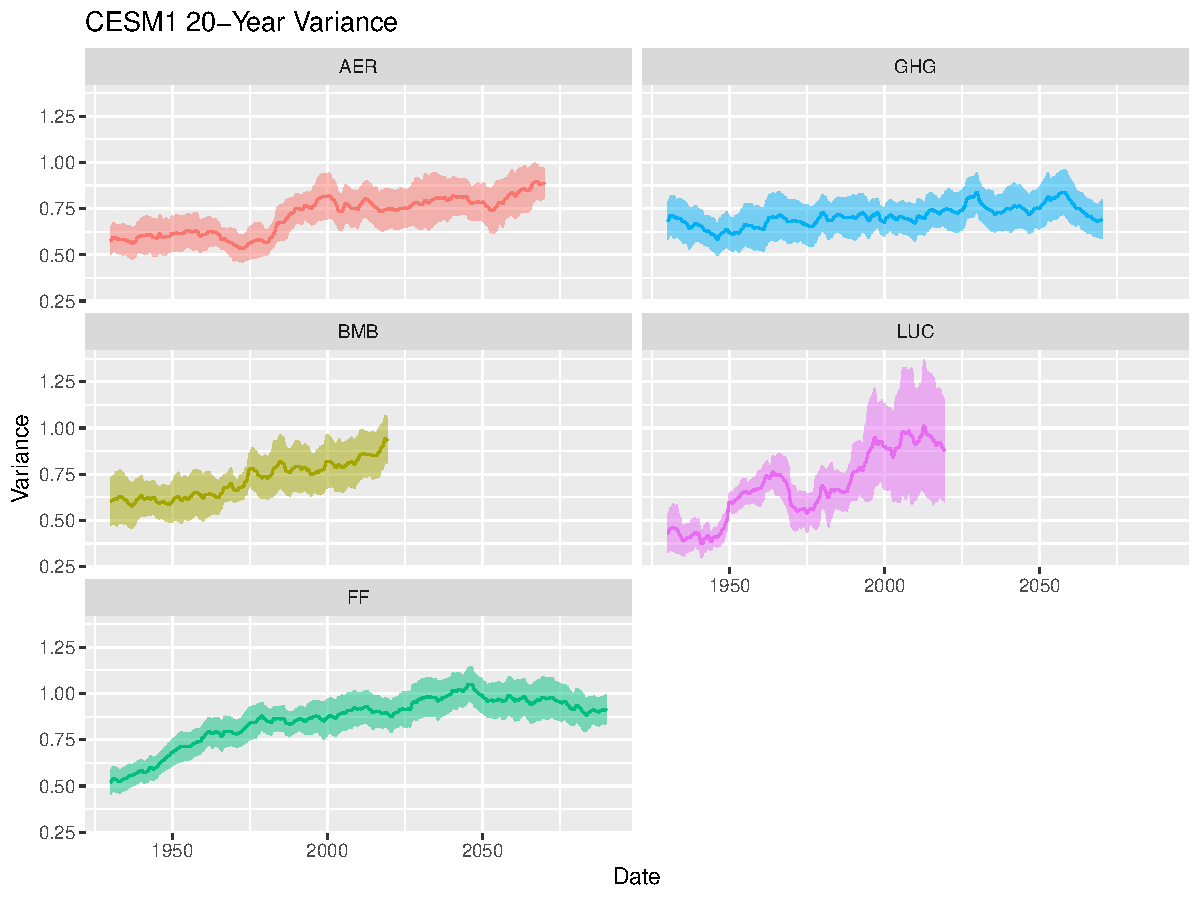
\includegraphics[width=.5\linewidth]{../../data/figures/cesm1.pdf}
\caption{\label{fig:variance_1}20-year windowed variance of the Niño 3.4 index, for ensembles a) full-forcing, b) xghg, c) xaer, d) xbmb, e) xlulc. Colored bars represent ensemble standard error.}
\end{figure}

\begin{figure}
\centering
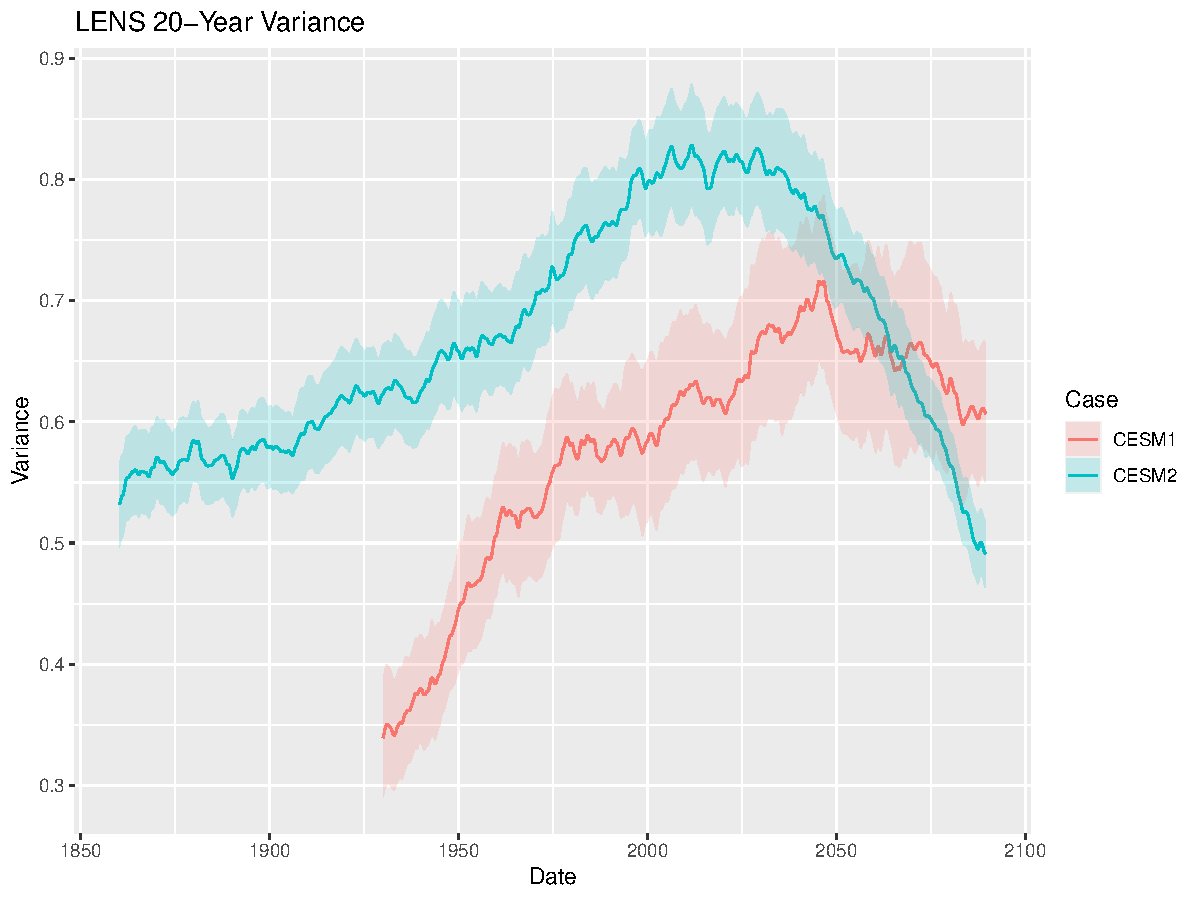
\includegraphics[width=.5\linewidth]{../../data/figures/ff_compare.pdf}
\caption{\label{fig:variance_2}20-year windowed variance of the Niño 3.4 index for the CESM1 and CESM2 fully-forced Large Ensembles. Colored bars represent ensemble standard error.}
\end{figure}


\subsection{Single Forcing Scenarios and the Bootstrap Process}

We analyze the role of individual factors using the CESM Single Forcing Ensembles. To separate the influence of a single factor from the fully-forced ensemble, we employ a bootstrap test. For each single-forcing ensemble, a single simulation is randomly selected, and the Niño 3.4 20-year variance record is subtracted from that from a randomly selected fully-forced simulation. We repeat this process 1000 times for each ensemble, and then calculate the mean and standard error for each ensemble. These results are shown in figure \ref{fig:bootstrap_1}. The greenhouse-only ensemble as well as the aerosol-only ensemble exhibit increased variance, signaling that greenhouse and aerosol emissions likely both play a significant role in ENSO's forced response in the full-forcing ensemble. Interestingly, the influence of greenhouse gasses and aerosols are non-conflicting, in contrast with previous studies that show opposite effects of greenhouse gas and aerosol forcing on ENSO \citep{stevenson2017forced}. All the other single forcing ensembles exhibit insignificant differences from the fully-forced ensemble. The biomass burning case shows very small deviations from the fully-forced case, while the ozone ensemble's period of recording is too small to draw meaningful conclusions. However, \citet{nowack2017role} showed that ozone forcing may dampen the effect of greenhouse-forced increases to ENSO amplitude by reducing changes to Pacific sea temperature and the Walker Circulation. The land use/cover case, while it does show large deviations from the fully-forced case, has an ensemble size (5 members) too small to lend any credibility to these changes.

In both the fully-forced scenario, and the greenhouse and aerosol only simulations, there is noticeably reduced Niño 3.4 variance in the mid-20\textsuperscript{th} century, below 2 standard errors of the control. We hypothesize that this discrepancy may be the result of anomalous initial conditions caused by internal variability of the control, as the control conditions are used to initialize all the forced runs. To test this hypothesis, we analyzed the impact of the Atlantic Multidecadal Oscillation (AMO) and the Atlantic Meridional Overturning Current (AMOC) on Niño 3.4 variance in the control simulation using records of the AMO and AMOC from the Climate Variability Diagnostics Package (CVDP) \citep{phillips2014evaluating}. We filtered the 20-year variance of the Niño 3.4 sea surface temperature in the control based on the strength of the AMO/AMOC, separating ENSO variance into groups where AMO < -1\(\sigma\), AMO < -2\(\sigma\), AMO > 1\(\sigma\), AMO >2\(\sigma\), and the same for AMOC. We then estimated the probability density function for each group using a kernel density estimator. We observed no consistent difference in the distribution of Niño 3.4 variance between any group. So far the question of reduced variance is unanswered, and it will be addressed in further depth later in the study.

\begin{figure}
\centering
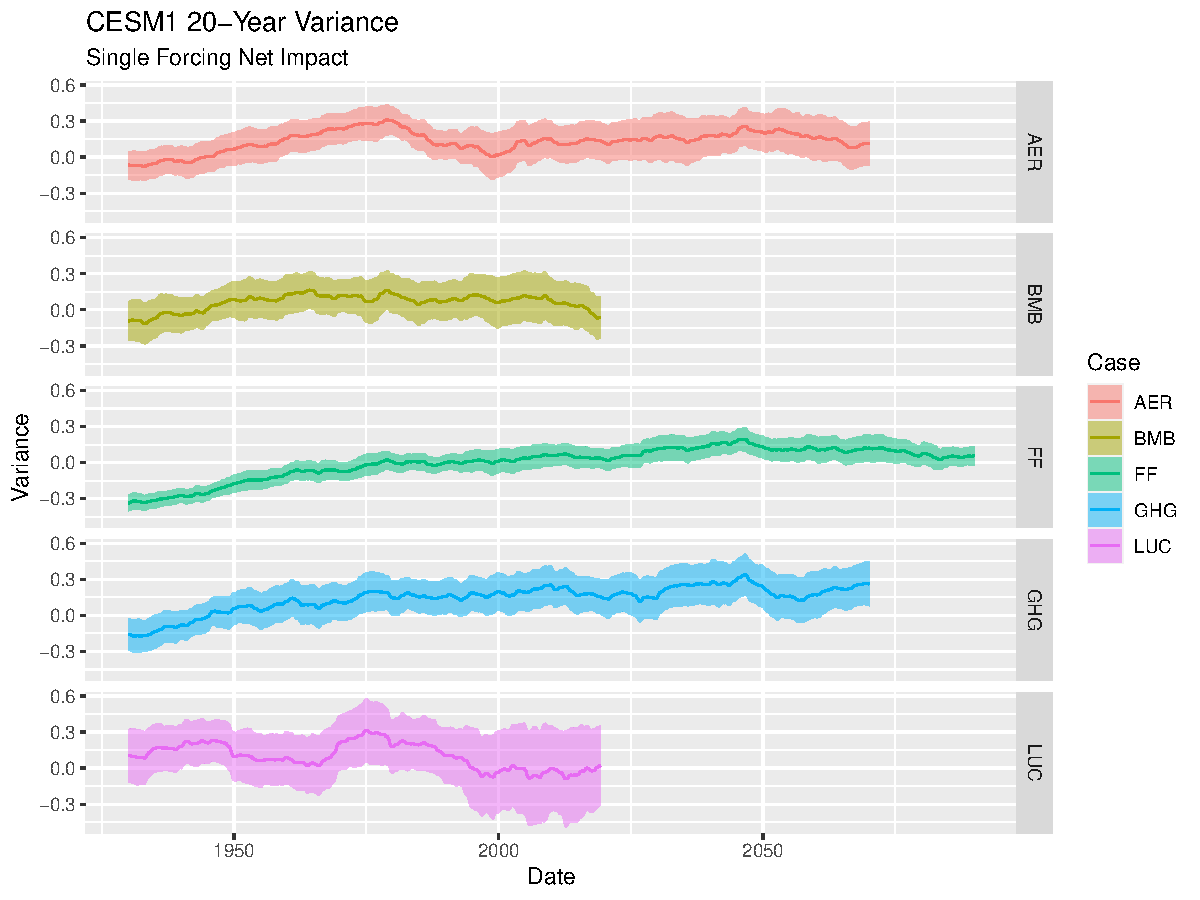
\includegraphics[width=.5\linewidth]{../../data/figures/cesm1_sf.pdf}
\caption{\label{fig:bootstrap_1}Difference between fully forced and single forced ensembles derived from the bootstrap process for a) aerosol emissions, b) biomass burning c) greenhouse gasses, d) land use/cover}
\end{figure}

\subsection{Correlation With Ocean Temperature}

Next, we analyzed the correlation between ENSO amplitude and changes to ocean structure in the CESM1 ensembles. To do this we used 4 slices of ocean temperature from the fully-forced, xghg, and xaer ensembles, including a slice averaged along the equator and slices through the western, central, and eastern Pacific basins. We linearly detrend and smooth with a 30-year windowed mean the timeseries at each grid-point and the Niño 3.4 variance. Next, we calculated the Pearson's correlation coefficient between each grid-point and the Niño 3.4 variance timeseries. The correlation coefficients for the equatorial slice are shown in figure \ref{fig:tempdt}.

Overall, the majority of the Pacific basin exhibits negative correlation with Niño 3.4 variance when linearly detrended and smoothed. The fully-forced simulation contains strongly negative correlation between the subsurface layer of the equatorial Pacific and ENSO amplitude, leading to the hypothesis that forced changes to Pacific Ocean stratification may be connected to ENSO intensity. However, it is unclear whether there is also a causal relationship between the two. Additionally, it is unclear whether the overall warming trend of the upper Pacific ocean is connected to changes to ENSO intensity. We notice that the high levels of correlation between the subsurface layer and Niño 3.4 variance are present in the xGHG and xAER ensembles, as well as the fully forced ensemble, suggesting that there is a relationship between ENSO amplitude and subsurface Pacific Ocean temperature in a variety of forcing scenarios.

\begin{figure}
\centering
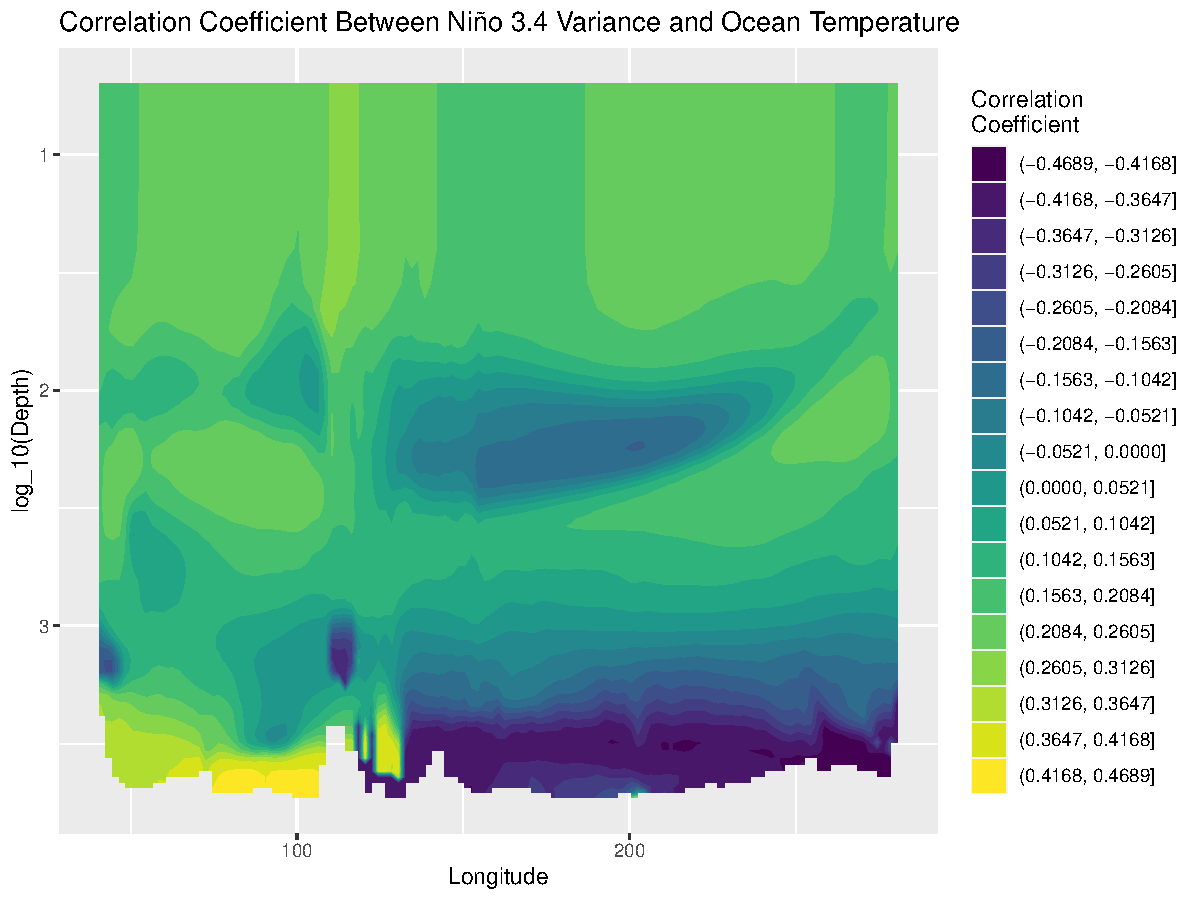
\includegraphics[width=.5\linewidth]{../../data/figures/tempdt.pdf}
\caption{\label{fig:tempdt}Correlation coefficient between detrended and smoothed ocean temperature averaged along the equator and detrended and smoothed Niño 3.4 variance.}
\end{figure}

\subsection{Wavelet Analysis}

Finally, we conduct a wavelet analysis of the Niño 3.4 index for the CESM1 and CESM2 Large Ensembles. Wavelet analysis separates a timeseries into time and frequency domains, displaying the amplitude for each frequency at each time step. The wavelet transform works by scaling a specified ``mother wavelet'' and translating it across the series at each scaling. This method is superior to a windowed Fourier Transform because it has high resolution on both time and frequency domains. First, we subtract the ensemble mean from each member and apply a 1-year windowed mean. Next, we construct a power spectrum of the Niño 3.4 index for each member following the methods of \cite{torrence1998practical} and calculate the ensemble mean of these power spectra, as displayed in figure \ref{fig:wavelet_2}. The majority of ENSO variability is contained in the 2 to 8-year frequency band. This band exhibits steadily increasing wavelet power until the mid 21\textsuperscript{st} century, conforming to previous results of this study. Both ensembles show an increase in the dominant ENSO signal, peaking in the 21\textsuperscript{st} century. The CESM2 ENSO amplitude peaks slightly earlier than the CESM1, in accordance with figure \ref{fig:variance_2}. The CESM2 exhibits a slight decrease in the dominant ENSO period during the 21\textsuperscript{st} century, with the mean power spectrum's ridgeline decreasing from a period of approximately 4 years to 2.5 years. It is unknown whether this period decrease is statistically robust. Finally, the CESM2 has a lower peak wavelet power than the CESM1, in contrast with that shown in figure \ref{fig:variance_2}.

To further examine the nature of forced changes to the ENSO spectrum, we split ENSO's power spectrum into two records for each ensemble, the two groups having periods less than and greater than 3 years. Then, we calculate the mean power along the time axis, effectively generating records of ENSO amplitude split into two frequency groups. Ensemble mean and standard error are found for each time-step. These records are shown in figure \ref{fig:wavelet_2}.

\begin{figure}
\centering
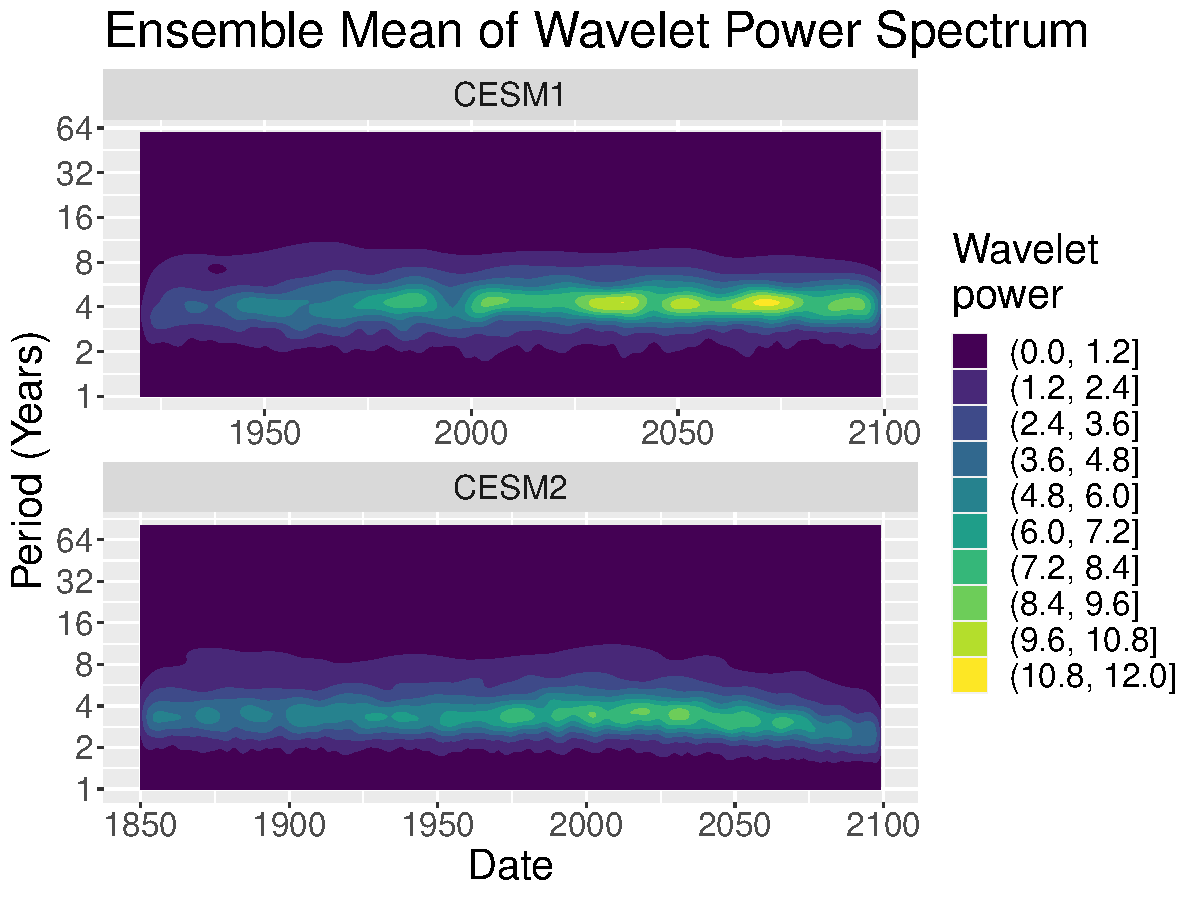
\includegraphics[width=.5\linewidth]{../../data/figures/wavelet2.pdf}
\caption{\label{fig:wavelet_1}Ensemble mean wavelet power spectra for both large ensembles.}
\end{figure}

\begin{figure}
\centering
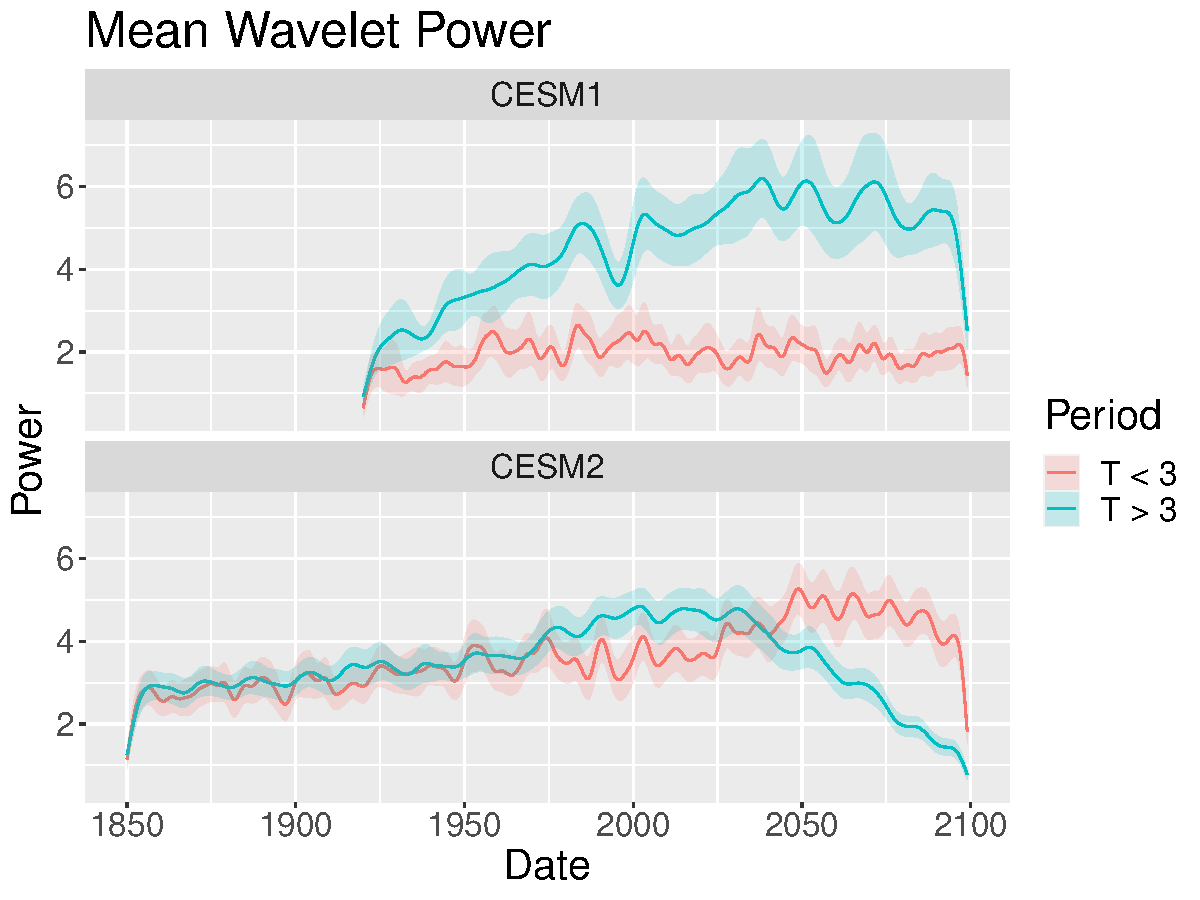
\includegraphics[width=.5\linewidth]{../../data/figures/wavelet3.pdf}
\caption{\label{fig:wavelet_2}Ensemble mean wavelet power records for low and high period ENSO.}
\end{figure}

\section{Conclusion}

In this study, predicted changes to ENSO amplitude are examined in the CESM1 Large Ensemble and Single Forcing Ensemble. The fully-forced large ensemble exhibits increased ENSO amplitude, as measured by calculating the 20-year variance of the Niño 3.4 index. These changes appear to be statistically significant, but need to be scrutinized further, as they are in disagreement with results of some previous studies \citep{stevenson2012significant}. Additionally, the fully-forced ensemble, as well as all the others contains considerable noise, as the individual members cover a wide range of variability. Greenhouse gas and aerosol emissions are likely the most significant contributors to these forced changes, as shown by the fact that the ensemble mean for the xGHG and xAER ensembles are the most different from the fully-forced mean. All the other single-forcing ensembles had insignificant differences from the fully forced ensemble, or were lacking a sample size large enough to lend credibility to their results. Analysis of the correlation coefficient between ENSO amplitude and Pacific ocean temperature reveals that changes to ENSO intensity are tied to changes to the subsurface layer of the tropical Pacific Ocean. It is still unclear what is driving this connection, as well as how external forcing such as global warming affects it. There has been shown to be a connection between Pacific stratification and ENSO variability as higher levels of stratification result in a stronger thermocline feedback, which causes the Pacific to become less stable, making strong ENSO events more likely \citep{dewitte2012reinterpreting}.

This study produced similar results as of previous studies, as it predicts an increase in ENSO amplitude, as well as overwhelming noise caused by internal variability \citep{maher2018enso}. Although there is limited research on the impact of individual external factors on ENSO, this study complements the results of \citet{stevenson2017forced}, who observed conflicting effects of greenhouse gas and aerosol emissions on ENSO diversity. In contrast, this study observes that the impact on ENSO amplitude of greenhouse gas and aerosols has the same sign. This result is also surprising given that greenhouse and aerosol emissions have been shown to have opposite effects on sea surface temperature and global circulation, with greenhouse emissions favoring a more Niño-like state with weakened Walker circulation and higher SST, and aerosol emissions counteracting these effects \citep{boer2000transient}.

This study has a number of goals for future continuation. The most pressing of these goals is a deeper analysis of changes to Pacific Ocean structure, which will be done by examining correlation between ENSO amplitude and potential density, as well as comparisons of changes to stratification in the Pacific. Additionally, the methods of this study will be repeated on the CESM2 large ensemble, which has a larger ensemble size and a longer record period, as compared to CESM1. Analysis of the CMIP6 models are also necessary to verify these results across variations in model physics. Deeper statistical analyses of changes to ENSO amplitude should also be tone to further examine the likelihood and intensity of future changes to ENSO amplitude. Lastly, correlation between ENSO amplitude and internal variability should be further investigated using the records provided by the CVDP. Doing these further analyses will help to verify the results of this study, while more precisely analyzing future changes to ENSO.

The results of this study will help to direct future studies on the impact of climate change on ENSO by providing one further data point supporting the conclusion that ENSO will intensify due to global warming. This study and others like it will help societies impacted by ENSO to prepare for intensification in the future.

\section{Acknowledgments}

This material is based upon work supported by the National Center for Atmospheric Research, which is a major facility sponsored by the National Science Foundation under Cooperative Agreement No. 1852977. Computing resources (\href{https://doi.org/10.5065/D6RX99HX}{doi:10.5065/D6RX99HX}) were provided by the Climate Simulation Laboratory at NCAR's Computational and Information Systems Laboratory, sponsored by the National Science Foundation and other agencies. I would like to thank Ms. Kimberly Fleming and the White Plains High School Science Research Program for providing support in this study.


\bibliographystyle{apalike}
\bibliography{references}
\end{document}
